O sistema proposto contempla o desenvolvimento de uma aplicação multiplataforma, composta por versões para web e dispositivos móveis, que atua como o principal meio de interação entre o usuário e os dados da propriedade. A aplicação oferece uma interface gráfica intuitiva, permitindo o acompanhamento completo das informações cadastradas e garantindo um controle preciso e em tempo real do rebanho, desde que a plataforma seja constantemente alimentada pelo usuário. Cada versão da aplicação desempenha um papel específico: a plataforma mobile, direcionada a funcionários e veterinários, prioriza a agilidade no lançamento de informações em campo; enquanto a versão web, voltada a gestores e proprietários, proporciona uma visualização mais ampla e detalhada dos dados em ambiente de escritório. Ambas atuam de forma integrada, promovendo sincronização automática e assegurando a consistência das informações em tempo real.

Conforme ilustrado no \Cref{fcht:fluxograma}, a interação com o usuário inicia-se nas etapas I e II. A etapa I corresponde à plataforma web, desenvolvida em \textit{React} com o framework \textit{Next.js}. Atualmente, a plataforma web encontra-se hospedada na Vercel, uma solução \textit{serverless}, que dispensa a necessidade de um servidor dedicado. A etapa II refere-se à plataforma mobile, desenvolvida em \textit{React Native}, framework que consiste em um conjunto de ferramentas voltadas à criação de aplicações móveis nativas \cite{Bruna2021}. O aplicativo tem como principal funcionalidade oferecer uma interface simplificada e intuitiva, voltada ao lançamento de dados em campo.

Ambas as plataformas comunicam-se com o Back-end (etapa III) por meio de uma Interface de Programação de Aplicações, do inglês \textit{Application Programming Interface} (API), desenvolvida em \textit{TypeScript} com o framework \textit{Nest.js}. Como parte do Back-end, foram implementados recursos adicionais com o objetivo de aperfeiçoar a usabilidade e a fluidez do sistema, destacando-se a integração com dois modelos de Inteligência Artificial(IA). A primeira delas é a API \textit{Gemini} (etapa IV), um modelo generativo multimodal desenvolvido pelo Google. No contexto deste projeto, a \textit{Gemini} é utilizada no sistema de alertas, por meio do modelo \textit{gemini-1.5-flash}. Essa implementação analisa um \textit{prompt} elaborado especificamente para o domínio do sistema e define a prioridade de cada alerta como alta, média ou baixa, simplificando de maneira significativa a lógica de priorização e resposta.

A segunda IA (etapa V) foi desenvolvida pelo próprio grupo e baseia-se no algoritmo \textit{Random Forest Regressor}, um método de aprendizado supervisionado que combina múltiplas árvores de decisão para realizar previsões numéricas. O modelo é treinado com diversas amostras aleatórias dos dados e, para cada árvore, um subconjunto de atributos, conhecidos como \textit{features}, é selecionado de forma aleatória, promovendo diversidade entre os estimadores. A predição final é obtida a partir da média dos resultados de todas as árvores, aumentando a precisão e reduzindo o risco de sobreajuste, conhecido como \textit{overfitting}, em comparação com o uso de uma única árvore de decisão. No contexto deste trabalho, o modelo tem como objetivo prever individualmente a produção de leite de cada fêmea, utilizando seu histórico produtivo, reprodutivo, sanitário, zootécnico e genético. Essas informações são consolidadas em um conjunto de \textit{features} estruturadas e, a partir delas, o sistema gera uma predição que classifica o potencial produtivo em categorias, sendo elas alto, bom, médio ou baixo. O resultado é ainda comparado com a média da propriedade e fornece informações adicionais, como o volume previsto em litros, o percentual em relação à média e a data da predição.

Para disponibilizar todo o Back-end de forma operacional e acessível, o mesmo foi hospedado na nuvem utilizando o serviço \textit{Amazon EC2}, \textit{Elastic Compute Cloud}, da \textit{Amazon Web Services} (AWS). Essa escolha permite escalar a infraestrutura dinamicamente, otimizando custos e garantindo melhor desempenho do sistema. A API é responsável por gerenciar toda a lógica de negócios, incluindo a criação, consulta, atualização e exclusão de registros no banco de dados, além de processar requisições provenientes das plataformas web e mobile. O controle de \textit{deploy} automático (etapa VI) é realizado por meio do \textit{GitHub Actions}, que integra diretamente com a instância EC2, automatizando atualizações e correções e assegurando que a aplicação permaneça sempre disponível e atualizada para os usuários.

Para o armazenamento das informações, o banco de dados do sistema (etapa VII) foi desenvolvido em \textit{PostgreSQL}, escolhido pela sua robustez e pela consistência oferecida pelo modelo relacional na organização e integridade dos dados. Essa estrutura permite armazenar grandes volumes de informações de forma estruturada, garantindo que registros relacionados, como dados de produção, lactação e histórico sanitário dos animais, sejam mantidos de forma segura e coerente. Atualmente, o banco de dados encontra-se hospedado na nuvem por meio da plataforma \textit{Supabase}, que oferece compatibilidade nativa com o PostgreSQL, além de recursos adicionais de autenticação e armazenamento.

\begin{flowchart}[!htb]
\centering
\caption{Arquitetura do fluxo das redes}%
\label{fcht:fluxograma}
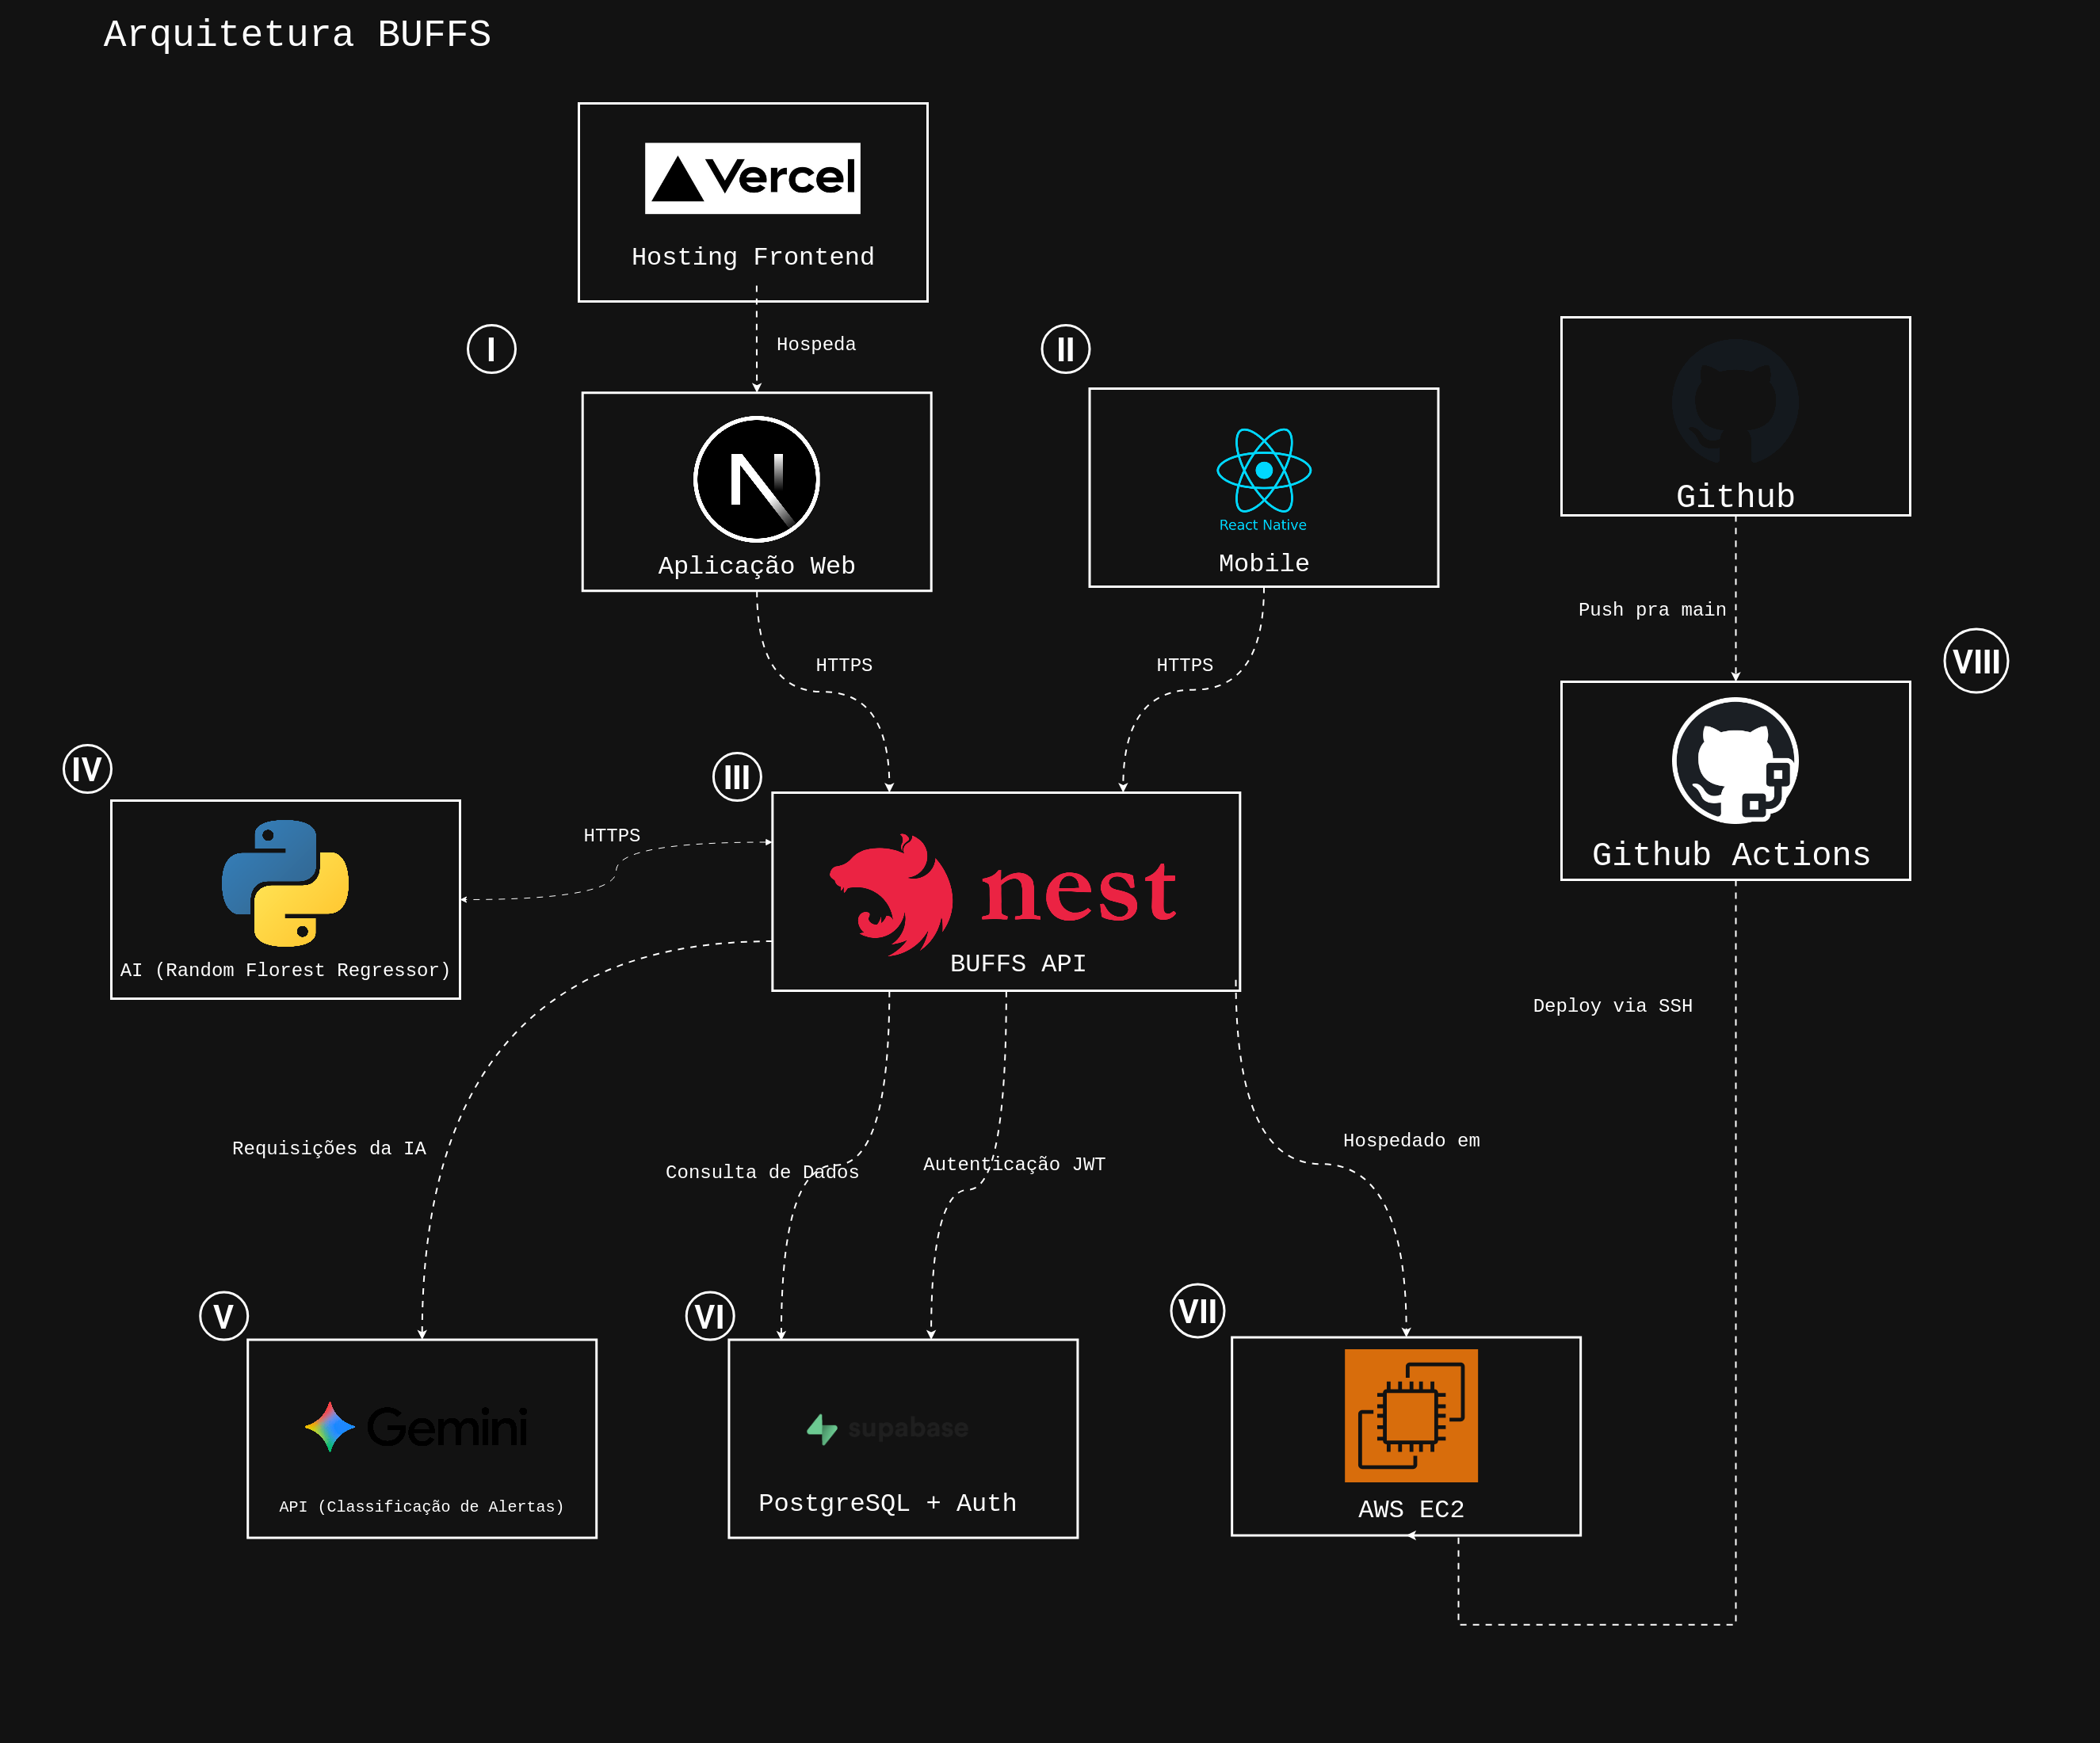
\includegraphics[scale=0.15]{buffs-arch-model}
\SourceOrNote{Autoria Própria (2024)}
\end{flowchart}

\newpage
Após a análise do fluxo apresentado, nota-se que grande parte do sistema encontra-se hospedada na nuvem, seja por meio de serviços \textit{serverless}, de bancos de dados em ambiente cloud ou de máquinas virtuais dedicadas. Essas escolhas, no momento atual, mostraram-se adequadas sob a ótica do grupo, uma vez que permitem distribuir as \textit{stacks} entre diferentes serviços, evitando a sobrecarga de um único sistema. Além disso, essa configuração possibilita a realização de testes de forma gratuita, sem a necessidade de investimentos iniciais em infraestrutura. Essa abordagem visa preparar o sistema para as próximas etapas do projeto, especialmente a fase de testes e validação da plataforma em um ambiente real, como uma propriedade rural parceira que venha a colaborar com o experimento. Após a conclusão da fase de validação, será possível mensurar o volume de recursos necessários para manter o sistema operacional de maneira estável, avaliando o custo-benefício e o dimensionamento adequado da infraestrutura, de modo a garantir a continuidade e o desempenho da aplicação.


